\chapter{Mini-Project A}
\label{sec:ProjA}
This project examines ELO5.2, which requires the student to develop a representative embedded system. It requires hardware/software interfacing, so an ADC is sampled by software, and processing operations are applied to read the data. 

\section{Project Requirements}
The Project is split into Milestones in order to help you plan time and ensure you aren't overburdened with work a few days before the final deadline. Dates for submission will be put on Vula. The milestones are as follows:
\begin{enumerate}
    \renewcommand{\theenumi}{\Alph{enumi}}
    \item Planning and System Design\\
    For this milestone we expect to see the following:
    \begin{itemize}
        \item A Gantt Chart indicating your planned activities with the project
        \item A circuit diagram for the system
        \item A choice on how you plan to approach the project (e.g. Spiral, waterfall, etc.) as well as a justification as why
        \item A flowchart detailing how the system operates
    \end{itemize}
    \item Code and Report\\
    The final hand in will be the report and your code submission. Details on these can be found in the marking guides.
\end{enumerate}

\section{Outcomes}
In addition to creating a working system, you will learn about the following in this project:
\begin{itemize}
    \item Technical outcomes
    \begin{itemize}
        \item ADC - \href{https://cdn-shop.adafruit.com/datasheets/MCP3008.pdf}{MCP3008}
        \item Temperature sensor - \href{http://ww1.microchip.com/downloads/en/devicedoc/20001942g.pdf}{MCP9700A}
        
    \end{itemize}
    \item Other outcomes
    \begin{itemize}
        \item Team Work
        \item Design methodologies, such as the Waterfall, Spiral and V Models.
        \item Planning and time management
    \end{itemize}
    
    
\end{itemize}

\section{Deliverables}
At the end of this project, you must:
\begin{itemize}
    \item Submit all milestones
    \item For information on the marks and what sections to cover, refer to the marking guide in Section \ref{sec:ProjAMarks}
\end{itemize}

\section{System Overview}
Figure \ref{fig:SystemOverview} shows the system overview for the mini-project.
\begin{figure}[H]
\centering
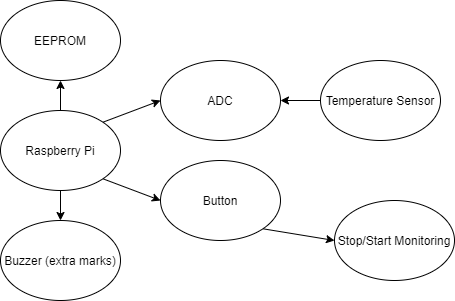
\includegraphics[width=0.6\columnwidth]{Figures/2020-SystemOverview-A}
\caption{Components of Mini-Project A}
\label{fig:SystemOverview}
\end{figure}

\section{Hardware requirements}
You will need to build your designed circuit on a breadboard and demonstrate it in the video you create.

\section{Software requirements}
You need to do the following:
\begin{itemize}
    \item Set up the EEPROM. 
    \item Create a thread for reading from the ADC. The value read from the temperature sensor needs to be converted to degrees Celsius. See the datasheet (linked above) for the formula.
    \item Create interrupts for all the button functionality (don't forget to debounce your inputs)
    \item Create an output signal to trigger the buzzer (bonus marks)
    \item In the main() loop, print values to the screen as described in Section \ref{sec:ProjDescription}
\end{itemize}

\section{Description}
\label{sec:ProjDescription}
\begin{itemize}
    \item By default, the system continuously monitors the sensors every 5s using this format:
    \begin{table}[H]
    \centering
    \begin{tabular}{|l|l|l|l|}
    \hline
    Time     & Sys Timer & Temp  &  Buzzer  \\ \hline
    10:17:15 & 00:00:00  & 25 C  & *        \\ \hline
    10:17:20 & 00:00:05  & 25 C  &          \\ \hline
    10:17:25 & 00:00:10  & 25 C  &          \\ \hline
    10:17:30 & 00:00:15  & 25 C  &          \\ \hline
    10:17:35 & 00:00:20  & 25 C  &          \\ \hline
    10:17:35 & 00:00:20  & 25 C  & *        \\ \hline
    \end{tabular}
    \end{table}
    \item The stop switch stops or starts the monitoring of the sensors. The system timer is not affected by this functionality. The screen must also be cleared when logging is stopped, and a message printed to display to inform the user that the logging has stopped.
\end{itemize}

\section{Marking Guide}
\label{sec:ProjAMarks}
\begin{longtable}[c]{|l|l|}
\caption{Project A marking Guide}
\label{tbl:ProjAMarks}
\\\hline
\textbf{Heading} & \textbf{Report} \\ \hline
\endfirsthead
%
\endhead
%
Introduction & \begin{tabular}[c]{@{}l@{}}Provide a short introduction ($\sim \frac{1}{2}$ page) to your project explaining your main\\ design choices and how the report has been structured \textbf{{[}15 marks{]}}\end{tabular} \\ \hline
Requirements & \begin{tabular}[c]{@{}l@{}}The requirements section should provide a refined UML Use Case\\ diagram of the system, according to your implementation, and any\\ accompanying text that is needed to clarify the requirements.\\ Highlight any departures or additions that you may have made compared to\\ the original project description given in this document. \textbf{{[}15 marks{]}}\end{tabular}  \\ \hline
\begin{tabular}[c]{@{}l@{}}Specification \\ and Design\end{tabular} & \begin{tabular}[c]{@{}l@{}}This section should provide a UML State Chart describing the main\\ operation. Add a UML class or deployment diagram (or other suitable\\ diagram) to indicate the structuring of your implementation (e.g. code\\ modules/classes you may be using). You don’t need to provide fine detail of\\ the system, the diagram(s) can be e.g. at the level of functions. You should\\also include a circuit diagram \textbf{{[}20 marks{]}}\end{tabular}  \\ \hline
Implementation & \begin{tabular}[c]{@{}l@{}}This section should give some snippets of important code and explanations for\\ this (or referring to particular functions in code files). The point here\\ is elaborating any parts of the State Chart that are not so straightforward\\ to turn into code. \textbf{{[}20 marks{]}}\end{tabular} \\ \hline
\begin{tabular}[c]{@{}l@{}}Validation and\\ Performance\end{tabular} & \begin{tabular}[c]{@{}l@{}}Provide at least a paragraph or two explaining the performance of the\\ system. A snapshot could be included and you could show test cases where\\ you have tested that the system works reliably (e.g. using a powersupply to set \\ the value given to the ADC). \textbf{{[}20} \textbf{marks{]}}\end{tabular} \\ \hline
Conclusion & \begin{tabular}[c]{@{}l@{}}Give a summary of the extent that the system was found to be successful.\\ Discuss if you think that a system working in this way might be\\ considered a potentially useful product. \textbf{{[}10 marks{]}}\end{tabular}  \\ \hline
References & Provide a few references if relevant.  \\ \hline
Total & 100 \\ \hline
\end{longtable}